\documentclass[11pt]{article}
\usepackage[utf8]{inputenc}
% \usepackage[brazilian]{babel}
\usepackage[french]{babel}

\usepackage{subfigure}
\usepackage{indentfirst}
\usepackage{graphicx}
\usepackage{xcolor}
\usepackage[cm]{fullpage}
\usepackage{hyperref}
\usepackage{listings}
\lstset{
  basicstyle=\footnotesize\ttfamily,
}

\newcommand*{\alert}[1]{\vspace{0.4cm}\colorbox{gray!60!white}{\parbox{0.92\linewidth}{{\centering \textbf{IMPORTANT!}\\}#1}}\vspace{0.4cm}}

\title{Guide d'utilisation de Nanvix: \\ Installation, Compilation, Mise en route et Débogage}

\author{Pedro H. Penna, Fernando Jorge Mota, Márcio Castro\\[0.2em]
  \small Universidade Federal de Santa Catarina (UFSC)\\[1.0em]
  Jean-François Méhaut\\[0.2em]
  \small Université Grenoble Alpes (UGA)\\
}
\date{}

\hyphenation{tool-chain}

\usepackage{url}

\begin{document}

\maketitle

\section{Introduction}

Avant de commencer les développements, il est essentiel de
vous familiariser avec l'organisation des fichiers du système Nanvix,
les outils de développement que vous allez utiliser et le processus de
génération du système. Pour cette première séance, vous travaillerez sur
toutes ces tâches et, à la fin, vous serez prêt à démarrer le travail
de développement.

Il est important de noter que les \textit{scripts} fournis pour
l'installation et l'exécution de Nanvix ont été testés sur les
distributions \textit{Ubuntu} et Lubuntu. Par conséquent, nous vous
recommandons fortement d'utiliser une de ces deux distributions
Linux. Nanvix peut certainement être compilé et exécuté avec d'autres
distributions Linux. Cependant, dans certains cas, vous devrez
apporter des modifications aux scripts d'installation pour les
adapter à votre distribution.

Pour démarrer, nous allons vous montrer comment télécharger le code
source de Nanvix et discuter de sa structure en répertoires (Section
~\ref{sec:code}). Ensuite, nous allons vous montrer comment installer
les outils de développement qui devront être compilés pour permettre
la génération du système (Section ~\ref{sec:tools}). Ensuite, nous
allons vous montrer comment compiler et mettre en route Nanvix
(Section ~ \ref{sec:compilation}). Enfin, nous montrerons un moyen
intéressant pour déboguer Nanvix en utilisant GDB (Section ~\ref{sec:debug}).
Enfin, nous allons montrer une alternative d'utilisation
de Nanvix avec l'utilisation de machines virtuelles (VMs) dans une
machine locale (Section ~ \ref {sec:vm}).

\section{Code source et la hiérarchie Nanvix}
\label{sec:code}

La première étape pour utiliser Nanvix est de télécharger le code
source. Pour ce faire, il suffit de cloner le dépôt de développement
comme suit \footnote {Si vous n'avez pas installé \texttt{git}, vous
  pouvez l'installer de la manière suivante: \texttt {sudo apt-get install git}} \\

\begin{lstlisting}[language=bash,numbers=none,frame=single]
git clone https://github.com/nanvix/nanvix
\end{lstlisting}

\vspace{0.3cm}

Dans le répertoire Nanvix, vous trouverez un certain nombre de
fichiers et de répertoires. Parce que le système d'exploitation Nanvix
couvre plusieurs aspects et qu'il est un peu complexe, Nanvix est
organisé autour d'une hiérarchie de répertoires, qui est détaillée
comme suit:

\begin{itemize}
\item \texttt{bin} contiendra le binaire du noyau \textit{kernel} et les
  utilitaires, une fois qu'ils auront été compilés.
  
\item \texttt{doc} contiendra la documentation de Nanvix avec des
  manuels sur le système, les bibliothèques, les utilitaires, les
  directives générales pour le développement ainsi que de la
  documentation des APIs.
  
\item \texttt{doxygen} contient des fichiers de configuration pour
  l'outil Doxygen qui permettront la génération de la documentation
  des APIs Nanvix directement à partir du code source.
  
\item \texttt{include} contient des fichiers .h de déclaration de
  constantes, de types et des prototypes des fonctions ou appels au
  système Nanvix.
  
\item \texttt{lib} contiendra les biblithèques statiques ou dynamiques,
  une fois qu'elles auront été compilées.
  
\item \texttt{src} contient le code source du noyau du système Nanvix
  ainsi que des utilitaires.
  
\item \texttt{tools} contient les procédures et les \textit{scripts}
  nécessaires à la compilation du système, des utilitaires ainsi que
  les bibliothèques statiques ou dynamiques.
\end{itemize}

\section{Environnements et outils de développement}
\label{sec:tools}

Les outils utilisés pour le développement du système Nanvix diffèrent
de ceux utilisés pour le développement logiciels plus classiques.

D'abord, les outils de génération doivent être compatibles avec la
plate-forme cible et son processeur. Par exemple, Nanvix a été conçu
pour la plate-forme de processeur Intel x86 (IA32 pour architectures
32 bits).  La conséquence est que les outils utilisés pour compiler le
système Nanvix doivent être capables de générer du code machine pour
cette plate-forme. Ensuite, lorsque vous travaillez au niveau du noyau
(\textit {kernel}), l'environnement de développement ne fournit aucun
type de bibliothèque standard. Enfin, pour tester le système Nanvix,
il faudra utiliser une machine dédiée, qu'elle soit réelle ou
virtuelle. Enfin, les outils pour la mise au point \textit{débogage}
disponibles sont d'assez bas-niveau, mais extrêmement puissants.

Pour le développement de nouvelles fonctionnalités pour Nanvix,
vous utiliserez deux outils:

\begin{itemize}
\item La \textit {toolchain} gcc-x86, une collection d'utilitaires qui
  inclut un compilateur (\textit{gcc}), un assembleur (\textit{as},
  et un éditeur de liens (\textit {linker}, \textit{ld});

\item Bochs, un émulateur de plate-forme Intel x86 doté d'un puissant
  \textit {debogeur} intégré.
\end{itemize}

Pour installer automatiquement ces outils, exécutez les commandes suivantes
avec un mode privilégié d'exécution (\texttt{sudo}). Il y a deux
scripts à exécuter qui sont dans le répertoire \texttt{tools/dev}.\\

\begin{lstlisting}[language=bash,numbers=none,frame=single]
sudo bash tools/dev/setup-toolchain.sh
sudo bash tools/dev/setup-bochs.sh
sudo reboot now
\end{lstlisting}

\vspace{0.3cm} Le processus de génération et d'installation des outils
peut prendre un certain temps (plusieurs minutes). Vous rebooterez
(\textit{reboot}) votre machine après l'installation des outils
de développement.

\section{Compilation et mise en route de Nanvix}
\label{sec:compilation}

A partir du moment où les outils pour compiler le Nanvix auront été
correctement installés, la compilation du système Nanvix devient une
tâche simple. En vous positionnant dans le répertoire racine du
projet, vous appelerez l'utilitaire \texttt {make} avec comme argument
\texttt {nanvix}. Une fois cette commande exécutée, tous les fichiers
binaires auront été créés avec succès.

Pour générer une image du système Nanvix, vous allez une nouvelle fois
appeler l'utilitaire \texttt {make} à partir du répertoire racine,
mais cette fois avec l'argument \texttt {image}. Cela va entraîner la
création du fichier \texttt {nanvix.img} dans le répertoire racine. Ce
fichier représente l'image système et sera utilisé dans la phase de
démarrage (\textit {boot}) décrite dans le paragraphe suivant.

\begin{lstlisting}[language=bash,numbers=none,frame=single]
make nanvix
make image
\end{lstlisting}

Enfin, vous allez démarrer le système Nanvix dans Bochs en invoquant
le \textit {boot} sur l'image système générée. Pour ce faire
automatiquement, exécutez, à partir du répertoire racine, le \textit
{script} \texttt {run.sh} situé dans le répertoire \texttt
{tools/run}.

\vspace{0.3cm}

La première commande compile le Nanvix. Une fois cette
commande terminé, tous les fichiers binaires doivent avoir été créés
avec succès. La seconde commande génère une image \footnote {Si vous
  utilisez la distribution \textit {Arch Linux}, vous devrez peut-être
  installer le paquetage \texttt {cdrtools} pour créer l'image. Pour
  ce faire, exécutez la commande suivante: \texttt {pacman -S
    cdrtools}} à partir du système, créant ainsi le fichier \ texttt
{nanvix.img} dans le répertoire racine. Ce fichier est l'image système
et sera utilisé dans le processus \textit {boot} ci-dessous.

Enfin, lancez le fichier dans \textit {Bochs}, en donnant \textit {boot} sur l'image système générée.
Pour ce faire automatiquement, exécutez la commande \textbf {suivante à partir du répertoire racine du projet}:
\\

\begin{lstlisting}[language=bash,numbers=none,frame=single]
bash tools/run/run.sh
\end{lstlisting}

\vspace{0.3cm}
En cas de succès, vous verrez Nanvix en cours d'initialisation (boot). Après l'initialisation, l'écran principal du terminal Nanvix est
prêt à l'emploi, comme illustré sur la figure ~\ref {fig:terminal-nanvix}.

\begin{figure}[t]
	\centering
	\subfigure[Après le démarrage (boot) de Nanvix]{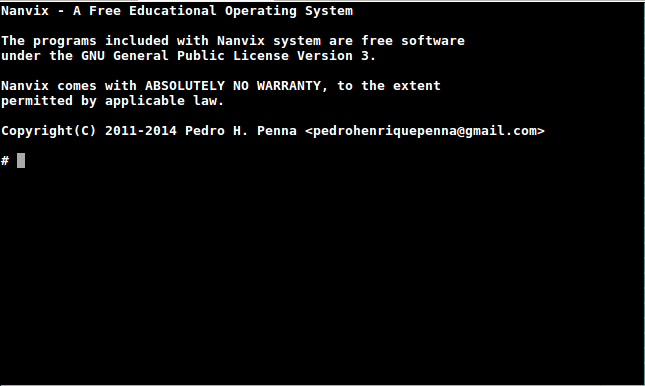
\includegraphics[scale=0.38]{img/terminal-nanvix.png}\label{fig:terminal-nanvix}}
	\subfigure[[GDB après un \textit {breakpoint} dans la fonction \texttt{yield} du \textit {kernel}.] {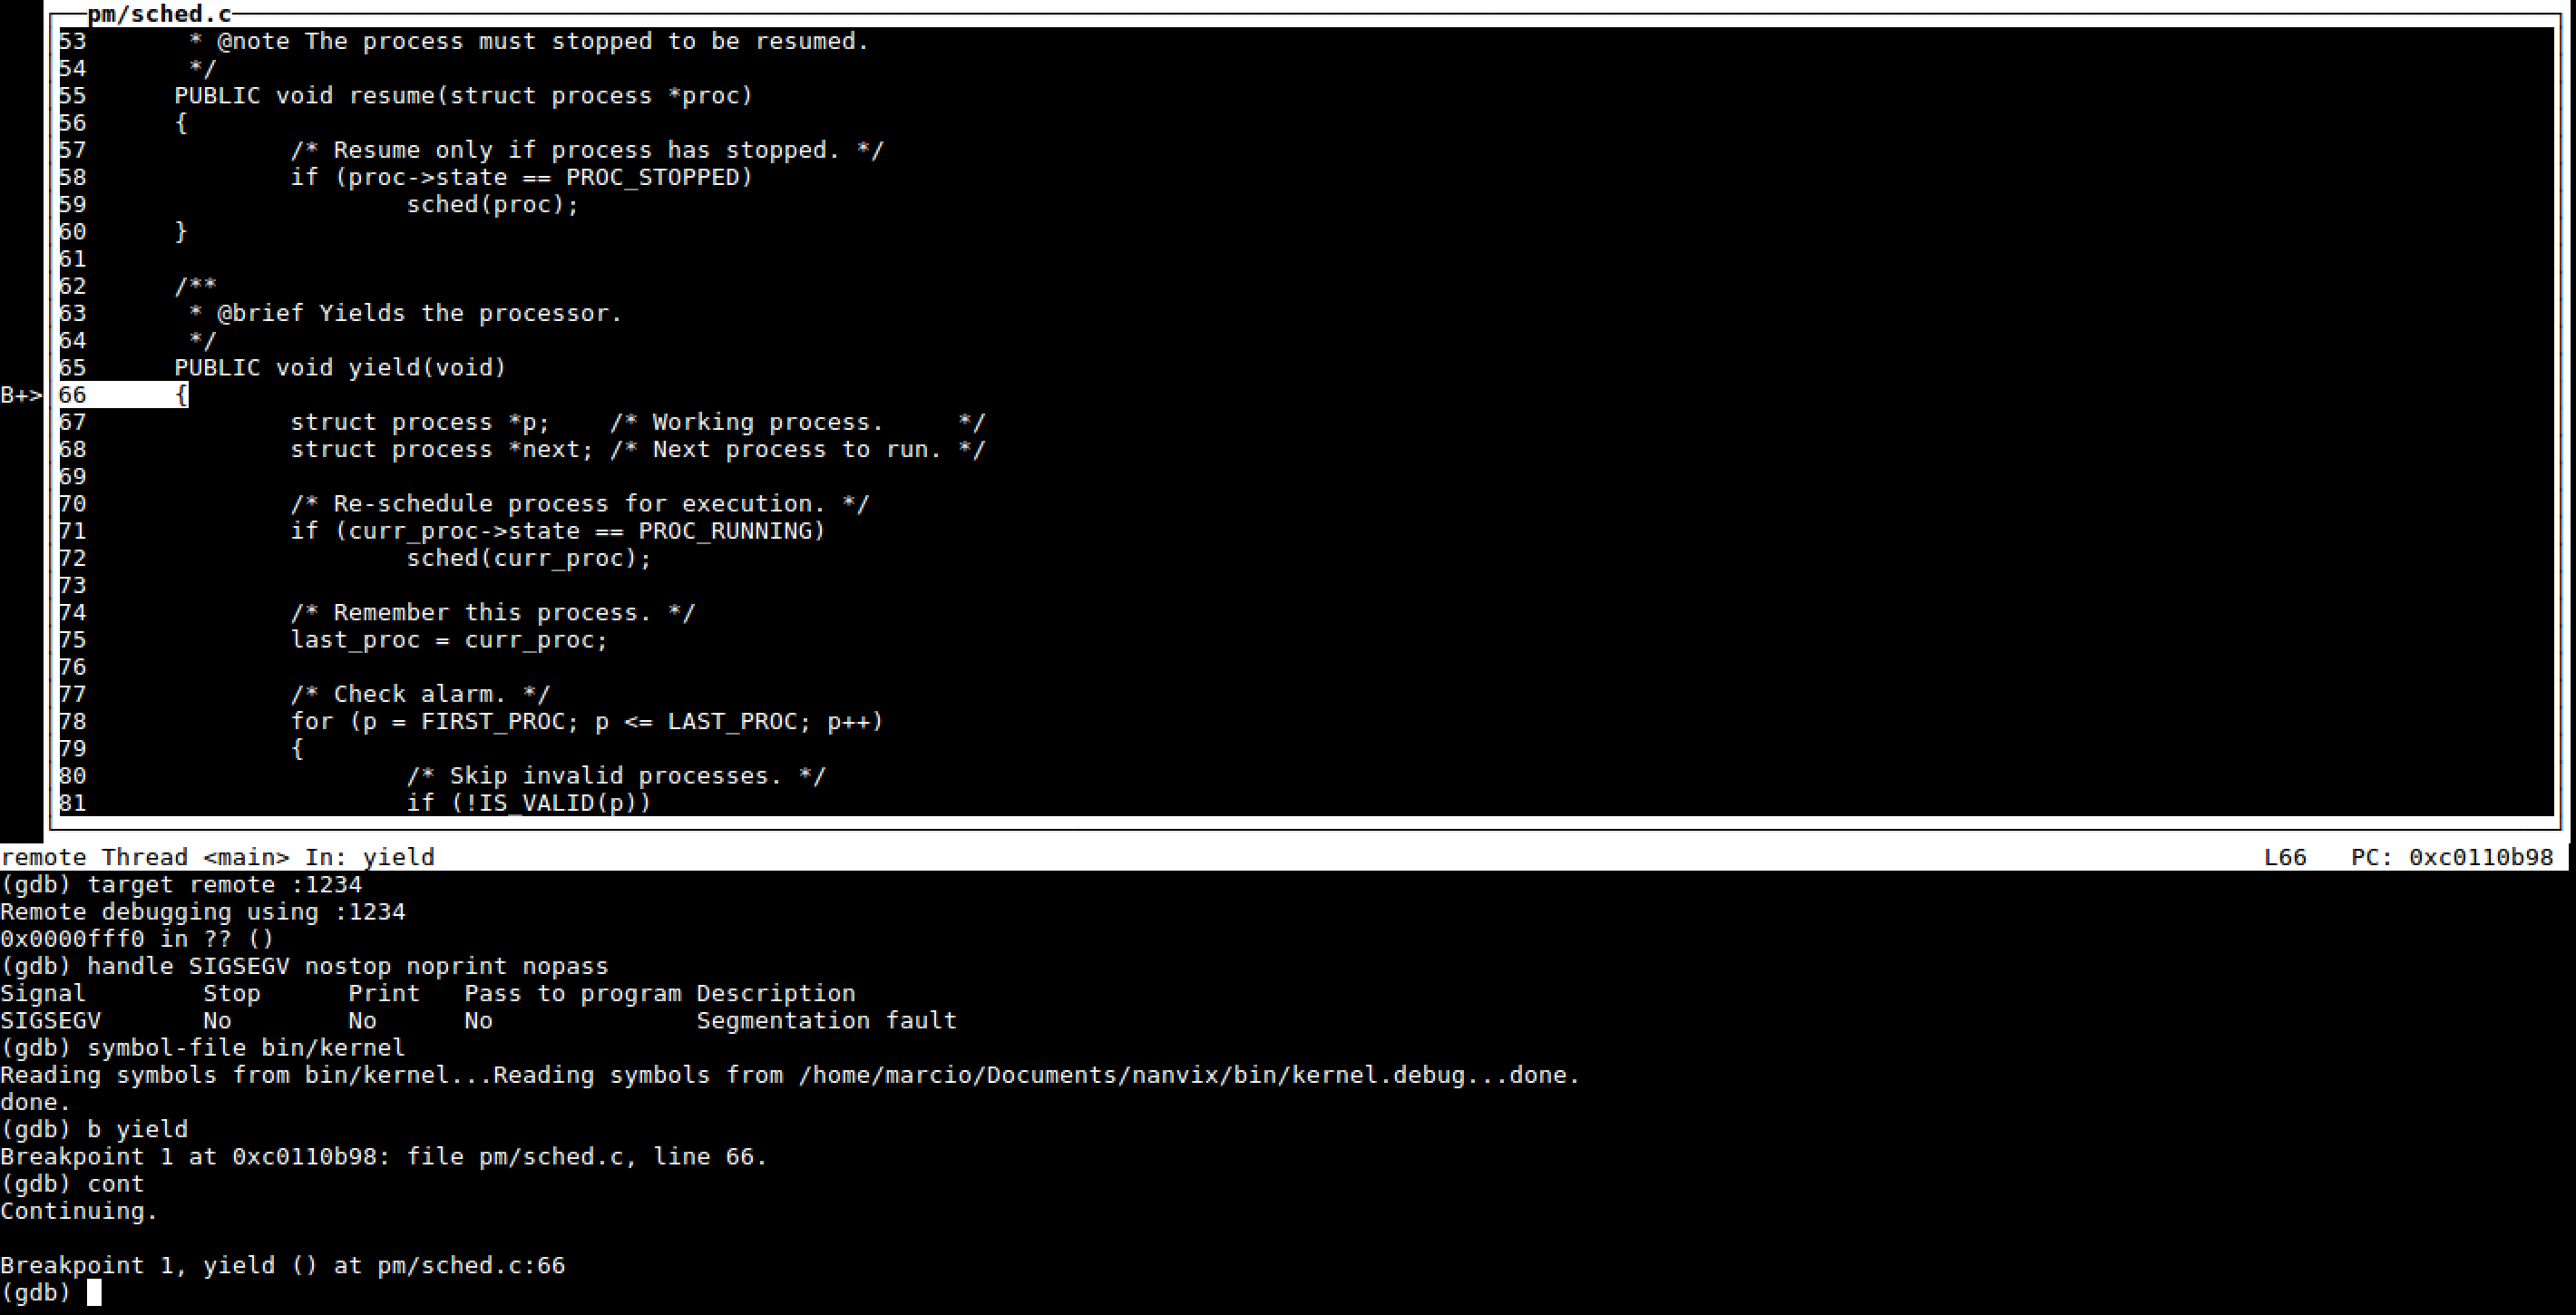
\includegraphics[scale=0.22]{img/terminal-GDB.png}\label{fig:terminal-gdb}}
\caption{Fenêtres avec Nanvix et GDB.}
\end{figure}

\alert{\textit {Bochs} sera exécuté directement dans le terminal. Pour
  terminer correctement l'exécution de l'émulateur \textit {Bochs},
  appuyez d'abord sur CTRL Z pour mettre en pause l'exécution du
  processus \textit {Bochs}. Ensuite, entrez la commande suivante sur
  le terminal pour terminer l'exécution de \textit {Bochs}: \texttt
  {kill -HUP \%1}.}.

\section{Débogage de Nanvix}
\label{sec:debug}



Pour déboguer Nanvix, qui peut être très utile pour identifier
et corriger des \textit{bogues} et autres problèmes qui se posent
dans le code en cours de développement \textit {noyau},
l'utilisation de GDB est nécessaire, l'utilisation et l'intégration
seront présentées dans la section actuelle. 

Pour exécuter en mode de débogage Nanvix et activer le support GDB
utiliser la commande suivante dans un terminal: \\

\begin{lstlisting}[language=bash,numbers=none,frame=single]
bash tools/run/run.sh --debug
\end{lstlisting}

\vspace{0.3cm}
Ensuite, démarrez GDB \textbf {sur un autre terminal} à
partir du répertoire racine du projet, en utilisant la commande
suivante: \\

\begin{lstlisting}[language=bash,numbers=none,frame=single]
gdb --tui
\end{lstlisting}

Le paramètre \texttt{-tui} est optionnel mais très intéressant. Avec
lui, vous activez la prise en charge d'une interface utilisateur en
mode texte pour afficher le code source pendant le débogage, comme
illustré dans la figure ~\ref{fig:terminal-gdb}.

Pour commencer le débogage, exécutez les commandes suivantes sur le
terminal GDB: \\

\begin{lstlisting}[language=sh,numbers=none,frame=single]
target remote :1234
handle SIGSEGV nostop noprint nopass
cont
\end{lstlisting}

\vspace{0.3cm}
Voici une brève explication des commandes données ci-dessus:

\begin{enumerate}
	\item Il se connecte au \textit{Bochs}, qui affichera  qu'un client est connecté;
	\item Définit que les défauts de page et autres interruptions
          fréquentes doivent être complètement ignorées par GDB. SIGSEGV
          est juste un alias pour représenter les autres interruptions qui
          sont normales pendant l'exécution de la machine;
	\item Définit la machine pour continuer à fonctionner.
\end{enumerate}

En cas de succès, vous verrez comment GDB est connecté à Bochs, comme
le montre la figure ~\ref{fig:terminal-gdb}. Après l'exécution de la
commande \texttt {cont}, le terminal Nanvix sera disponible sur
l'écran Bochs et GDB sera bloqué. Pour relâcher le terminal GDB,
appuyez sur \textbf {CTRL C} sur le terminal GDB. De cette façon,
GDB va à nouveau interrompre l'exécution de Nanvix et permettre le
contrôle de l'exécution en mode \textit {debug} via GDB.

Lors de la compilation de Nanvix, plusieurs fichiers contenant les
tables de symboles du \textit {kernel} et des programmes système et
utilisateur ont été créés. Cependant, ces tables de symboles ne sont pas
chargées automatiquement. Pour charger la table de symboles contenant
des informations sur toutes les fonctions de \textit {kernel}, vous
pouvez utiliser la commande: \\

\begin{lstlisting}[language=sh,numbers=none,frame=single]
symbol-file bin/kernel
\end{lstlisting}

\vspace{0.3cm}
D'autre part, si votre objectif est de déboguer un
programme spécifique s'exécutant au dessus de Nanvix, il sera
nécessaire de charger la table de symboles du programme désiré. Par
exemple, pour charger la table de symboles du programme, tapez le
chemin d'accès à l'exécutable dans le dossier \texttt {bin}: \\

\begin{lstlisting}[language=sh,numbers=none,frame=single]
symbol-file bin/ubin/ls
\end{lstlisting}

\alert{Il n'est pas recommandé d'utiliser plus d'une table de symboles
  à la fois, car GDB ne sera pas capable de différencier les symboles
  correctement. Ainsi, lorsque vous exécutez cette commande sur un
  terminal où la table de symboles de \textit {kernel} a déjà été
  chargée, GDB demandera si la table de symboles doit être remplacée,
  ce qui est nécessaire pour déboguer un programme Nanvix.}

Pour insérer des \textit {breakpoints} (points d'arrêt), vous pouvez
utiliser la commande \texttt {b} \textbf {après le chargement de la
  table de symboles}.  Pour déboguer la fonction texttt {yield}, par
exemple, vous pouvez simplement faire: \\

\begin{lstlisting}[language=sh,numbers=none,frame=single]
b yield
\end{lstlisting}

\vspace{0.3cm}
À la place du nom de la fonction, vous pouvez également définir une ligne
où GDB doit définir \textit {breakpoint}. De cette façon, vous pouvez
utiliser la commande suivante pour définir un \textit {breakpoint}
sur la ligne 143 du fichier \textbf {main.c}, de la manière suivante: \\

\begin{lstlisting}[language=sh,numbers=none,frame=single]
b main.c:143
\end{lstlisting}

\vspace{0.3cm}
Notez que le \textit {breakpoint} ne fonctionne correctement uniquement
si vous chargez la table de symboles à l'aide de la commande
\texttt{symbol-file} précédemment spécifiée, car c'est à partir de la table
de symboles que GDB peut identifier les fichiers et fonctions concernées.

Après avoir positionné un \textit {breakpoint}, vous pouvez utiliser la
commande \texttt {cont} pour informer GDB qu'il doit s'arrêter lorsque
la prochaine occurrence de \textit {breakpoint} précédemment positionnée
est rencontrée. Ensuite, à partir d'un point d'arrêt donné, vous pouvez
utiliser la commande \texttt {step} pour passer à l'instruction suivante: \\

\begin{lstlisting}[language=sh,numbers=none,frame=single]
step
\end{lstlisting}

\vspace{0.3cm}
Vous pouvez également ignorer un certain nombre d'instructions en utilisant un paramètre optionnel de \texttt {step}. Par exemple, utilisez la commande suivante pour ignorer 10 instructions uniques: \\

\begin{lstlisting}[language=sh,numbers=none,frame=single]
step 10
\end{lstlisting}

\vspace{0.3cm}
La commande \texttt {step} vous permet d'effectuer un débogage de type \textit {step-by-step}. Cela signifie que lorsqu'une fonction est appelée pendant le
débogage, GDB ignore la première instruction de la fonction. Si vous voulez
passer directement à la fonction return avant de l'appeler, vous pouvez
utiliser la commande \texttt {next}: \\

\begin{lstlisting}[language=sh,numbers=none,frame=single]
next
\end{lstlisting}

\vspace{0.3cm}
En outre, pendant la phase de débogage, il est
intéressant d'utiliser la commande \texttt {print} pour imprimer les
variables qui pourraient être utiles pour comprendre l'exécution du
code. Ainsi, pour imprimer la variable globale \texttt {curr\_proc}, qui
est présente dans le Nanvix \textit {kernel}, vous pouvez utiliser: \\

\begin{lstlisting}[language=sh,numbers=none,frame=single]
print curr_proc
\end{lstlisting}

De même, vous pouvez utiliser une partie de la syntaxe C pour explorer
les différents attributs (champs) que la variable peut avoir. Par exemple,
pour imprimer le champ \texttt{pid} de \texttt {curr\_proc}, faites: \\

\begin{lstlisting}[language=sh,numbers=none,frame=single]
print curr_proc->pid
\end{lstlisting}

\vspace{0.3cm}
La commande ci-dessus imprime le PID (\textit{Process IDentifier})
du processus en cours d'exécution (dans le cas de Nanvix, le PID
est un attribut de \texttt{curr\_proc}).  Notez que \texttt {print}
fonctionne aussi sur \textit {breakpoints}, avec des variables locales,
il est donrc très utile de comprendre le comportement du code.

Enfin, pour visualiser la pile des appels de fonctions, vous pouvez
utiliser la commande \texttt {bt}, qui affiche le \textit {back-trace}
actuel du code: \\

\begin{lstlisting}[language=sh,numbers=none,frame=single]
bt
\end{lstlisting}

\vspace{0.3cm} Pour plus d'informations sur GDB, consultez le manuel à
l'adresse: https://sourceware.org/gdb/current/onlinedocs/gdb/

\alert{\textit{Bochs} ne supporte pas certaines opérations GDB,
  comme par exemple \texttt {watch} (pour suivre la valeur
  d'une variable dans le temps), ou les appels de fonction dans
  la commande \texttt{print}. Cela entraîne une erreur, une instabilité du
  système ou les deux. Par conséquent, leurs utilisations ne sont pas
  recommandées.}

\section{Nanvix dans une machine virtuelle (VM)}
\label{sec:vm}

Si vous n'avez pas de machine Linux et que vous ne voulez pas
l'installer directement sur votre machine, vous pouvez installer Linux
dans une machine virtuelle (VM) fonctionnant sur un autre système
d'exploitation (par exemple, Windows). Dans ce cas, nous vous
recommandons d'utiliser \textit {Virtual Box} (disponible sur
\url{www.virtualbox.org}). Après avoir installé Virtual Box, nous vous
conseillons d'installer Lubuntu 16.04 (disponible sur
http://lubuntu.net) sur VM, car il s'agit d'une distribution
relativement légère et testée. Enfin, il suffit de suivre les étapes
d'installation et de compilation (Sections ~\ref{sec:code} et
\ref {sec:compilation}) de Nanvix dans Ubuntu.

\end{document}
